\documentclass[a4paper,12pt]{article}
\usepackage{graphicx}
\begin{document}
\author{}
\title{Harvest Requirements and Design Documentation}
\maketitle
\center{\textbf{Team Name:} Binary Ninjaz\\}
\center{\textbf{Team Members:\\} 
Teboho Mokoena (u14415888)\\
Sizo Duma (u15245579)\\
Letanyan Delon Arumugam (u14228123)\\
John Ojo (u15096794)\\
Kevin Reid (u15008739)\\
Shaun Yates (u16007493)\\ }

\newpage{
\center{\textbf{Introduction}\\ 
	\flushleft{
The goal of the project is to design and develop a software system to be used by the farming community in the facilitation and management farming. The software system in development (Harvest) will be consisting of: an Android application, iOS application, and a website.
\newline\newline}

\center{\textbf{Functional Requirements:}}
\flushleft
  \item[$\bullet$]On sign in Harvest shall verify credentials against the database before signing them in. 
  \item[$\bullet$]Harvest shall create a profile on the database for the user through a registration form.
  \item[$\bullet$]Harvest shall measures yield, by combining a clocking system with yield data, through the input view of the mobile interface.
  \item[$\bullet$]The Harvest mobile interface shall make use of GPS data and based on weight and location assumptions, it must give approximate yield estimates not only for each orchard, but for each approximate location where the data was entered.
  \item[$\bullet$]The Harvest mobile interface shall make use of analytics to measure worker performance.
  \item[$\bullet$]The Harvest website shall display data on the farm on a heat map.
  \item[$\bullet$]The Web interface shall show detailed information about produce. (e.g. cultivar, year planted)
  \item[$\bullet$]The Harvest system shall track the foreman through their phone/tablets GPS.
  \item[$\bullet$]The Harvest system shall do administrative tasks through the web interface.
  \item[$\bullet$]The Harvest website shall give the farmer/administrator a real time map view of the foreman's location.
	
}
\newpage{
\center{\textbf{The Domain Model}\\ 
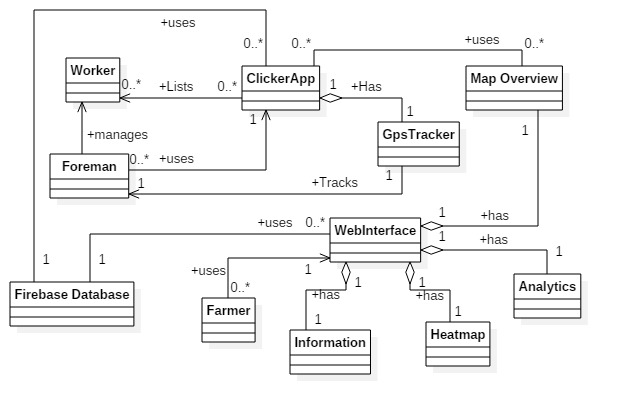
\includegraphics[width=1.2\linewidth]{actualDomain.jpg}
\center{\textbf{Architectural Design Process}\\ 
\flushleft{
  The architectural structural design of our the Harvest system is a Persistence Framework. The system has 3 main subsystems (Android Application, IOS Application and the website) all heavily reliant on the database system providing them with efficient object storage and retrieval without the need for implementation detail. 
}

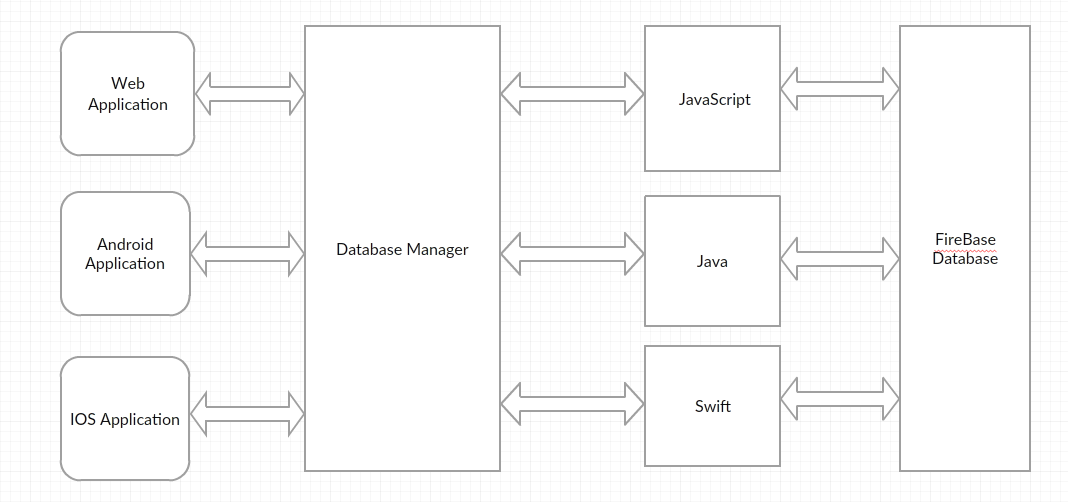
\includegraphics[width=1.0\linewidth]{persistenceFrameWork.PNG}

\center{\textbf{Deployment Diagram}\\ 
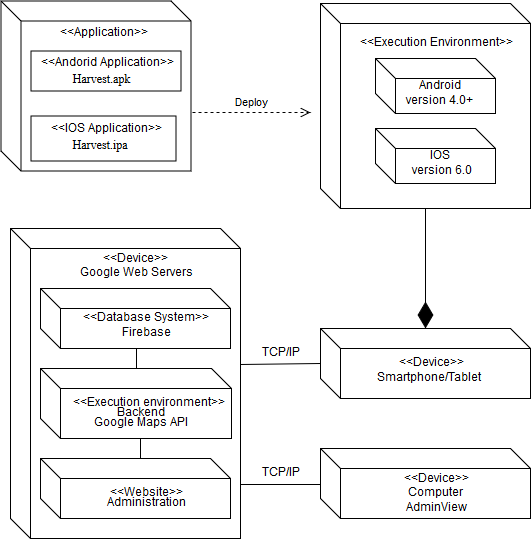
\includegraphics[width=.85\linewidth]{deployment.png}
}
	\subsubsection{Determining Design Objectives}
\flushleft
		\item[$\bullet$] The design is aimed to provide accessibility, data integrity and optimize performance.
		\item[$\bullet$] The design is also aimed at producing a user friendly easy to use system.
		\item[$\bullet$] The design is aimed at easing facilitation and automation of work. \newline\newline

	\center{\subsubsection{Determining Type of System}}
\flushleft
		The system under development is identified as an Object persistence subsystem (also known as a Database subsystem), because heavily focuses on  efficient information storage and retrieval . It also hides the database details such as implementation from the subsystems, and  therefore uses an abstract interface to manipulate data.
		
	\center{\subsubsection{Specifying Subsystem Functions, Interfaces, and Interaction Behaviour}}
\flushleft
		\item[$\bullet$]\textbf{The Application Interface: }This interface will have the functionality for login in and signing up of foremen. It will have yield data recording functionality and worker performance capturing functionality.
		\item[$\bullet$]\textbf{The Web Application Interface: }The administrative tasks will be carried out on the Interface (Like adding worker and Orchard Details per farm), as well as tracking of workers and performance.
		\item[$\bullet$]\textbf{The Database Interface: }This interface will maintain strict access, it will only be accessed through an abstract interface (Backend) only to store and retrieve data. \newline\newline
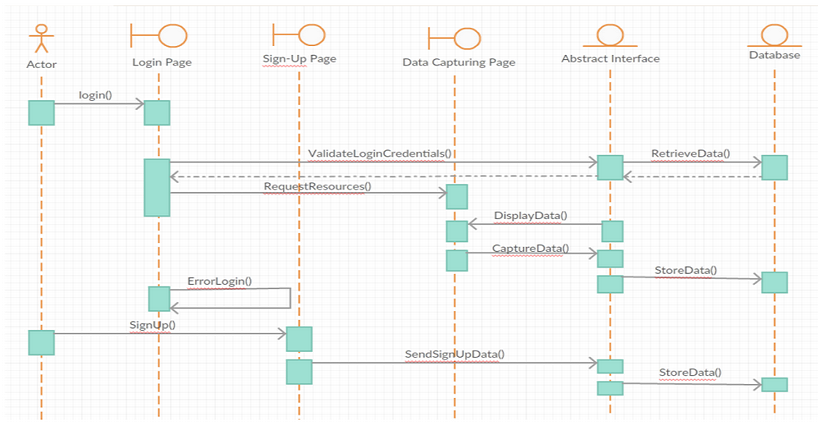
\includegraphics[width=1.2\linewidth]{sequenceDiag.PNG}
	\center{\subsubsection{Reviewing the architectural design}}
    \flushleft
		\item[$\bullet$]The Harvest application is accessible from a smartphone/tablet/desktop computer.
		\item[$\bullet$]The Harvest system checks whether the user is registered before signing them in. 
		\item[$\bullet$]Harvest creates a new profile of the user when registering them.
		\item[$\bullet$]Harvest does measures yield, by combining a clocking system with yield data, through the input view of the mobile interface.
		\item[$\bullet$]Harvest does facilitate GPS data filtering and Web Functionality
		\item[$\bullet$]The software application does facilitate the idea of tracking
		
		\center{\subsubsection{Technology Used}}
       \flushleft
		\item[$\bullet$]Database System : Firebase
		\item[$\bullet$]IDE's: Xcode, Android studio
		\item[$\bullet$]Programming languages: XML (Android UI); Java (Android Backend); Swift (IOS); HTML, CSS, JavaScript (Website)
}


\end{document} 

